
\section*{CHƯƠNG 1 - TỔNG QUAN ĐỀ TÀI }
\addcontentsline{toc}{section}{\numberline{}CHƯƠNG 1 - TỔNG QUAN ĐỀ  TÀI}
\setcounter{section}{1}
\setcounter{figure}{0}
\setcounter{table}{0}
\subsection{Bối cảnh và tầm quan trọng của Network Automation}
    Trong bối cảnh chuyển đổi số diễn ra mạnh mẽ, hạ tầng mạng doanh nghiệp ngày càng trở nên phức tạp với quy mô mở rộng không ngừng. Các tổ chức hiện đại thường phải quản lý hàng trăm đến hàng nghìn thiết bị mạng phân tán trên nhiều địa điểm khác nhau, từ router, switch đến firewall và các thiết bị bảo mật. Phương pháp quản trị mạng truyền thống dựa vào cấu hình thủ công qua giao diện dòng lệnh (CLI) không chỉ tốn thời gian mà còn tiềm ẩn nhiều rủi ro về sai sót do con người, đặc biệt khi thực hiện các thao tác lặp đi lặp lại trên nhiều thiết bị cùng lúc.
     \begin{figure}[H]
            \centering
            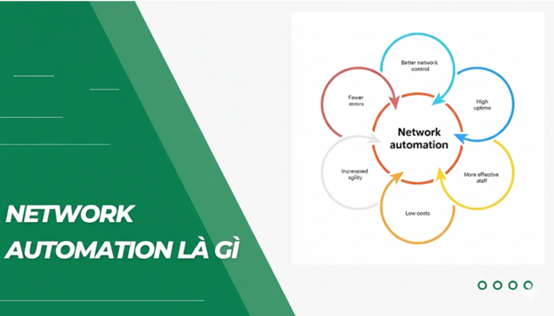
\includegraphics[width=0.7\textwidth]{image/Net_Auto.png}
            \caption{Tự động hóa mạng}
    \end{figure}

    Tự động hóa mạng (Network Automation)\cite{GeeksforGeeks-OSPF} xuất hiện như một giải pháp tất yếu để đáp ứng nhu cầu vận hành hạ tầng mạng hiệu quả, đáng tin cậy và có khả năng mở rộng cao. Thông qua việc sử dụng các công cụ lập trình và kịch bản tự động, quản trị viên mạng có thể triển khai cấu hình đồng loạt, giám sát trạng thái thiết bị theo thời gian thực, và phát hiện cũng như khắc phục sự cố một cách nhanh chóng. Điều này không chỉ giảm thiểu thời gian downtime mà còn tối ưu hóa nguồn lực nhân sự, cho phép đội ngũ IT tập trung vào các nhiệm vụ chiến lược thay vì các công việc lặp đi lặp lại.
    
    Hơn nữa, tự động hóa mạng đóng vai trò quan trọng trong việc đảm bảo tính nhất quán của cấu hình trên toàn bộ hệ thống. Khi các thay đổi được thực hiện thông qua script được kiểm thử kỹ lưỡng, khả năng xảy ra lỗi cấu hình giảm đáng kể so với việc nhập lệnh thủ công. Điều này đặc biệt quan trọng trong môi trường doanh nghiệp nơi mà sự cố mạng có thể gây ra thiệt hại tài chính lớn và ảnh hưởng nghiêm trọng đến hoạt động kinh doanh.

    

\subsection{ Mục tiêu nghiên cứu và phạm vi đề tài:}
\subsubsection{Mục tiêu nghiên cứu:}
Các mục tiêu chính, bao gồm:
\begin{itemize}
    \item \textbf{Mục tiêu học thuật:} Đề tài hướng đến việc nghiên cứu và phân tích các phương pháp tự động hóa trong quản trị hạ tầng mạng doanh nghiệp, từ đó đóng góp vào việc hệ thống hóa kiến thức về ứng dụng ngôn ngữ lập trình Python trong lĩnh vực network automation. Nghiên cứu tập trung vào việc đánh giá hiệu quả của các thư viện Python phổ biến như Netmiko, Paramiko trong việc tương tác với thiết bị mạng\cite{CloudMyLab-2025}, đồng thời xây dựng khung lý thuyết về quy trình tự động hóa từ thu thập thông tin, triển khai cấu hình đến giám sát và khôi phục hệ thống.Đề tài cũng tìm hiểu sâu về các giao thức mạng thiết yếu như VLAN, OSPF và cơ chế định tuyến động, phân tích cách thức tích hợp chúng vào một hệ thống tự động thống nhất. Thông qua việc thiết kế và triển khai mô hình thực nghiệm, nghiên cứu sẽ đưa ra các đánh giá khách quan về độ tin cậy, khả năng mở rộng và hiệu suất của giải pháp tự động hóa so với phương pháp quản trị thủ công truyền thống.
    \item \textbf{Mục tiêu kỹ thuật:}Về mặt kỹ thuật, đề tài xây dựng một hệ thống tự động hóa hoàn chỉnh trên nền tảng mô phỏng GNS3-VM\cite{GNS3-Homepage} với cấu trúc mạng gồm ba router và ba switch, mô phỏng môi trường doanh nghiệp quy mô vừa và nhỏ. Hệ thống được phát triển với các module chức năng chính bao gồm:
    Module cấu hình VLAN tự động: Triển khai phân đoạn mạng logic, cấu hình trunk port và access port theo từng yêu cầu nghiệp vụ cụ thể.
    Module định tuyến động OSPF\cite{Cisco-OSPF-7039-1}: Tự động thiết lập các thông số OSPF, quảng bá mạng và tối ưu hóa bảng định tuyến giữa các router.
    Module quản lý địa chỉ IP\cite{GeeksforGeeks-ClassfulIP}: Tự động gán và quản lý không gian địa chỉ IP trên các interface, đảm bảo tính nhất quán và tránh xung đột.
    Module thu thập thông tin thiết bị: Tự động truy vấn và lưu trữ thông tin về phiên bản IOS, cấu hình hiện hành, trạng thái interface và các metric quan trọng.
    Module phát hiện và khôi phục lỗi: Xây dựng cơ chế so sánh cấu hình thực tế với cấu hình chuẩn, tự động phát hiện sai lệch và thực hiện rollback hoặc remediation khi cần thiết.
    Module báo cáo và logging: Tự động sinh báo cáo dưới dạng CSV, TXT với đầy đủ thông tin về quá trình thực thi, kết quả và lỗi phát sinh.
    Toàn bộ hệ thống được thiết kế theo kiến trúc modular, dễ bảo trì và có khả năng mở rộng cho các chức năng nâng cao trong tương lai như tích hợp API RESTful hoặc giao diện web-based management.

    \item \textbf{Mục tiêu ứng dụng:} Về mặt ứng dụng thực tiễn, đề tài cung cấp một giải pháp cụ thể giúp các doanh nghiệp vừa và nhỏ tối ưu hóa quy trình quản trị mạng, giảm thiểu thời gian và chi phí vận hành. Hệ thống tự động hóa cho phép quản trị viên mạng triển khai hàng loạt thay đổi cấu hình trên nhiều thiết bị đồng thời, giảm đáng kể nguy cơ lỗi do con người  và rút ngắn thời gian downtime trong quá trình bảo trì.
    
    Giải pháp đặc biệt hữu ích trong các tình huống như triển khai nhanh chi nhánh mới, thay đổi cấu trúc VLAN theo yêu cầu nghiệp vụ, hoặc khôi phục hệ thống sau sự cố mạng. Khả năng tự động sinh báo cáo chi tiết giúp đáp ứng yêu cầu về kiểm toán, tuân thủ quy định  và hỗ trợ việc ra quyết định dựa trên dữ liệu.
    
    Hơn nữa, đề tài tạo ra một framework có thể tùy biến và mở rộng, cho phép doanh nghiệp điều chỉnh theo nhu cầu đặc thù của mình hoặc tích hợp vào các hệ thống quản lý tập trung (NMS) hiện có. Mô hình này cũng có thể được sử dụng làm công cụ đào tạo cho kỹ thuật viên mạng mới, giúp họ làm quen với các khái niệm network automation và Infrastructure as Code (IaC).

\end{itemize}

\subsubsection{Phạm vi đề tài:}
    Nghiên cứu được giới hạn trong môi trường mô phỏng GNS3-VM\cite{GNS3-Documentation} với thiết bị Cisco IOS, tập trung vào các giao thức và công nghệ phổ biến trong doanh nghiệp SME. Đề tài không bao gồm các khía cạnh bảo mật nâng cao, giám sát hiệu năng thời gian thực hoặc tích hợp với hệ thống cloud.

\subsection{Công nghệ sử dụng:}
    Để hiện thực hóa các mục tiêu đã đặt ra, đề tài lựa chọn và tích hợp một số công nghệ then chốt tạo thành một hệ sinh thái hoàn chỉnh cho tự động hóa mạng. Python được chọn làm ngôn ngữ lập trình chính nhờ vào tính đơn giản, dễ học và đặc biệt là hệ sinh thái thư viện phong phú trong lĩnh vực network automation. Python cung cấp khả năng xử lý chuỗi mạnh mẽ, hỗ trợ đa luồng, và có thể tích hợp dễ dàng với nhiều hệ thống khác nhau.
    
    Thư viện Netmiko đóng vai trò cốt lõi trong việc thiết lập kết nối và tương tác với các thiết bị mạng. Được xây dựng dựa trên thư viện Paramiko, Netmiko cung cấp một lớp trừu tượng cao hơn, được tối ưu hóa đặc biệt cho việc làm việc với các thiết bị network như Cisco, Juniper, Arista và nhiều nhà sản xuất khác. Thư viện này hỗ trợ nhiều phương thức kết nối an toàn thông qua SSH, cho phép gửi lệnh, nhận kết quả, và xử lý các tình huống đặc biệt như enable mode, config mode một cách tự động.
    
    Về mặt môi trường mô phỏng, GNS3-VM được sử dụng để tạo ra một môi trường lab ảo hóa hoàn chỉnh\cite{GNS3-Homepage}. GNS3 cho phép mô phỏng các thiết bị mạng thực tế với đầy đủ tính năng của Cisco IOS và các hệ điều hành mạng khác, mà không cần đến phần cứng vật lý đắt tiền. Nền tảng này cung cấp khả năng thiết kế topology linh hoạt, kết nối các thiết bị ảo với nhau, và quan trọng là cho phép các script Python kết nối đến các thiết bị này thông qua mạng IP ảo, tạo ra môi trường thử nghiệm gần giống với hệ thống thực tế.

    Sự kết hợp giữa Python, Netmiko và GNS3 tạo thành một giải pháp toàn diện, cho phép phát triển, thử nghiệm và triển khai các kịch bản tự động hóa mạng trong môi trường kiểm soát. Điều này không chỉ giảm thiểu rủi ro mà còn tạo cơ hội học hỏi và thử nghiệm các kỹ thuật mới một cách an toàn.

